\documentclass[a4paper]{article}

%% Language and font encodings
\usepackage[english]{babel}
\usepackage[utf8x]{inputenc}
\usepackage[T1]{fontenc}

%% Sets page size and margins
\usepackage[a4paper,top=3cm,bottom=2cm,left=3cm,right=3cm,marginparwidth=1.75cm]{geometry}

%% Useful packages
\usepackage{amsmath}
\usepackage{graphicx}
\usepackage[colorinlistoftodos]{todonotes}
\usepackage[colorlinks=true, allcolors=blue]{hyperref}

\title{Paper on sub-tree embeddings/similarity}
\author{Wei Zhong}

\begin{document}
\maketitle

\section{Introduction}

Tree isomorphism problem is a well studied problem set, it is methods of comparing and matching labeled trees in general. \cite{Valiente01anefficient} focuses on subtree matching and a bottom-up tree distance to measure tree similarity. Different from tree edit distance where measurement calculates the set of minimal operations needed to transform between trees (also called mapping, but only in ordered tree). 
Actually measurement such as edit distance for unordered trees (NP-complete \cite{ZHANG1992133}) and \textit{Alignment distance} \cite{JIANG1995137} (score sum of all opposing labels) for ordered tree (MAX SNP-hard) are not suitable to apply into math-aware search where efficiency plays a very important role.

\begin{figure}
\centering
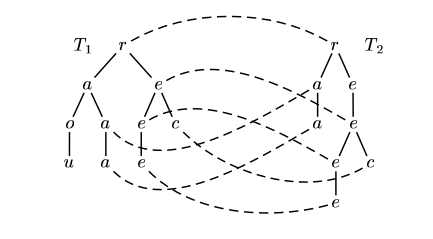
\includegraphics[width=0.5 \textwidth]{a.png}
\caption{\label{aaa} Sample isolated-subtree mapping which is neither top-down nor bottom-up.}
\end{figure}

\subsection{Relation to math search query autocompletion}
Math-aware search query autocompletion is different to other query autocompletion in a sense that math expression semantic structure is important, and query autocompletion needs to not only address query log frequency but also the importance of math expression structure similarity. Since many tree isomorphism problem is well studied and there are some tree distance measurement proposed, it is wise to research on these theory papers and utilize existing results to consider the possibilities to achieve efficient and well defined math expression similarity, thus will help math query autocompletion more relevant in terms of structural similarity.

\section{Bottom-up distance}
A bottom-up mapping between two trees is special case of \textit{isolated-subtree mapping}\cite{TANAKA} where the mappings always map between disjoint subtrees.
Bottom-up mapping is an isolated-subtree mapping in which children of nodes in the mapping are also in the mapping. And bottom-up distance is the bottom-up mapping of largest size.
This implies that bottom-up mapping only consider ``entire subtree" embedding where node outdegree must agree and thus graph in \ref{aaa} is not a bottom-up mapping.
An expected $O(n_1 + n_2)$ time algorithm has been introduced before to calculate bottom-up distance but \cite{Valiente01anefficient} has advanced the time complexity to maximum $O(n_1 + n_2)$ compared to his previous algorithm.

\subsection{Computation}
The largest bottom-up mapping between trees corresponds to the largest common forest between the two trees. The overall computation of the bottom-up distance is divided into several steps, first a compacted Directed acyclic graph is constructed. This DAG can be seen easily by drawing the two trees by height, such as:
\begin{verbatim}
(height 9) 11
(height 8) 12
(height 7) 13
(height 6) 1
(height 5) 20
(height 4) 6
(height 3) 2 14
(height 2) 3 7 9 15 18 22 24
(height 1) 4 5 8 10 16 17 19 21 23 25
\end{verbatim}
and then, collapsing all nodes at the same height into a single vertex.

Secondly, extract a mapping from two trees, and finally apply the mapping to \textit{distance} algorithm to compute bottom-up distance. The mapping algorithm extracts the mapping by going from bottom-up (level order) and find the node of its leftmost (in terms of preorder) counterpart in same height, and map the children of the two nodes in preorder. And the bottom-up distance is merely use the mapping to get what nodes are left unmapped and what mapped nodes does not have the same label, then use the specified weight to calculate the distance by summing them.

\bibliographystyle{alpha}
\bibliography{sample}

\end{document}
